\section{Einarbeitung}
In der Einarbeitungsphase haben wir uns zunächst für eine Hadoop-Arbeitsumgebung entschieden. Da die meisten Projektteilnehmer über lediglich vier Gigabyte Arbeitsspeicher verfügen, fiel unsere Wahl auf die ressourcenschonende Hortonworks Sandbox \footnote{Siehe: \url{http://hortonworks.com/products/hortonworks-sandbox/}}, die bei allen Teilnehmern problemlos ausgeführt werden konnte. Unter Verwendung der Sandbox haben wir den Umgang mit dem Hadoop-Ecosystem gelernt und erste Map/Reduce-Jobs ausgeführt. Darüber hinaus konnten wir weitere Tools wie Hive und Pig verwenden.

\subsection{Datenmodell}
Abbildung \ref{fig:ShoppersTables} zeigt das Datenmodell, dass aus den Entitäten transactions, history, offers, und submissions besteht...
\todo[inline]{Grafik passt nicht: trainHistory und testHistory berücksichtigen!}
\begin{figure}[h]
\centering
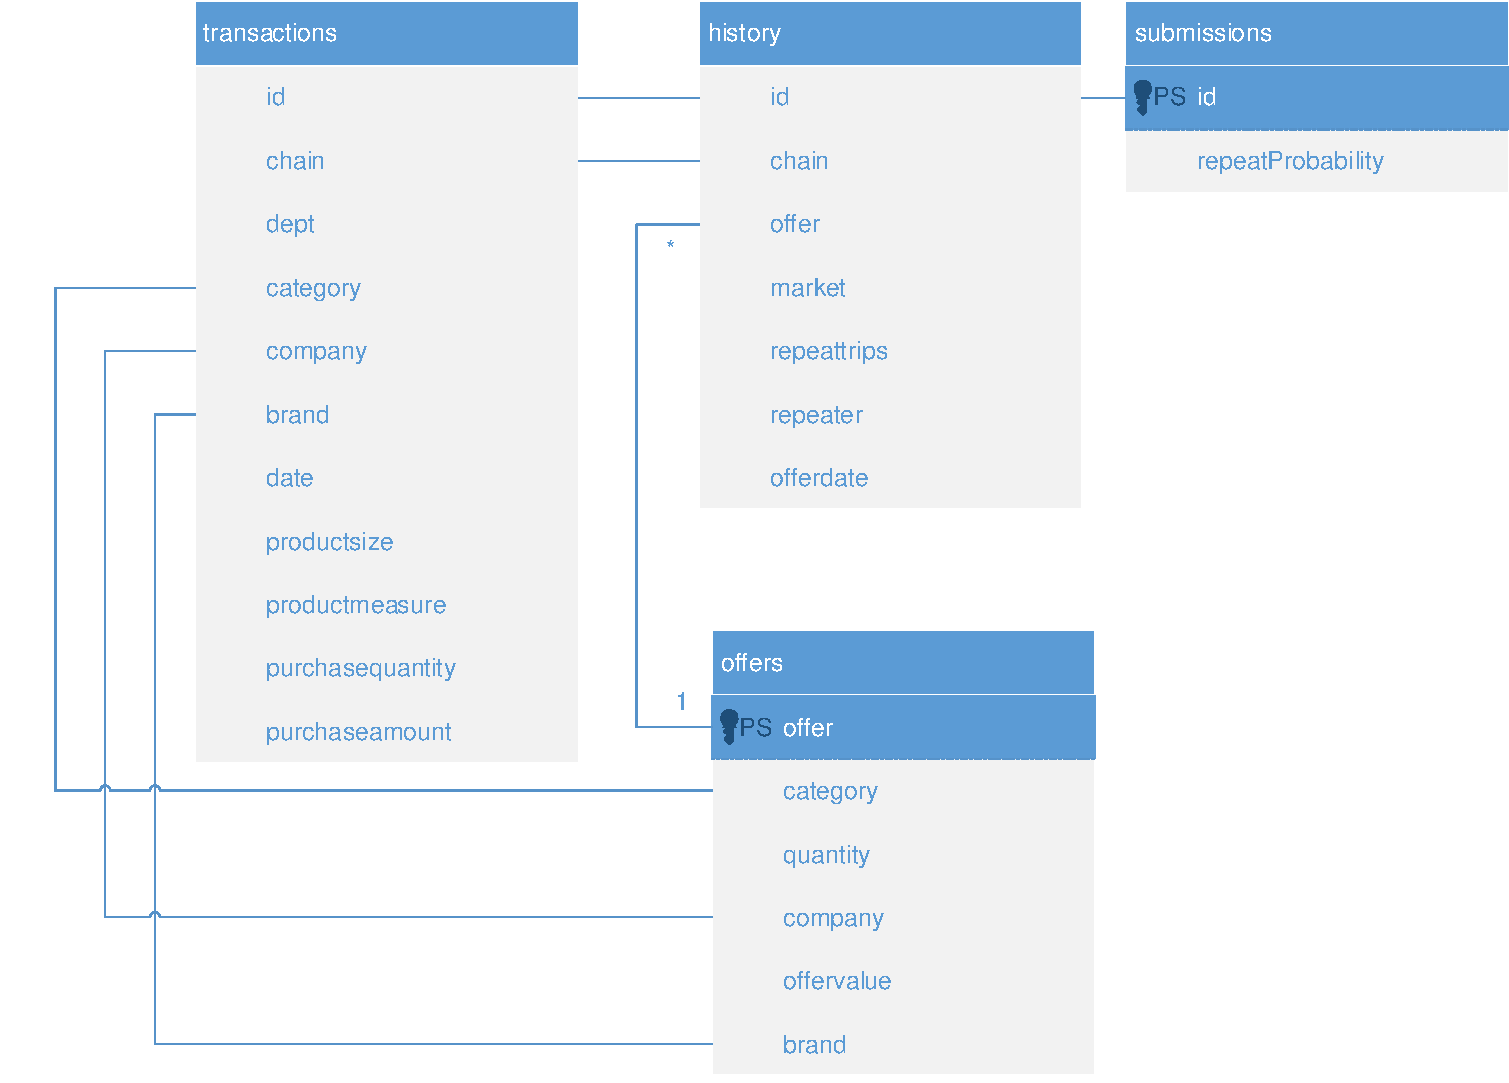
\includegraphics[width=0.7\linewidth]{Bilder/ShoppersTables}
\caption{Das Datenmodell}
\label{fig:ShoppersTables}
\end{figure}


\subsection{Technologieentscheidung}
Zu Beginn des Projekts haben wir uns Gedanken über die Auswahl der Technologien gemacht. Zum Zeitpunkt der Einarbeitungsphase haben wir bereits Hive und Pig durch gruppenübergreifende Vorträge kennen gelernt. Darüber hinaus standen uns keine weiteren Optionen zur Verfügung, da alternative Technologien erst zu einem späteren Zeitpunkt vorgestellt worden sind.

Somit beschränkte sich die Technologieentscheidung auf die Wahl zwischen Hive und Pig. Da wir in unserem Projekt ausschließlich Analysen auf strukturierte Daten durchgeführt haben, fiel unsere Entscheidung auf Hive. Der einfache Datenimport in Form von Tabellen und die einfachen Abfragemöglichkeiten in der SQL ähnlichen Abfragesprache HQL waren die ausschlaggebenden Kriterien.

Die Technologien, die wir neben Hive verwendet haben, werden im weiteren Verlauf der Dokumentation erläutert.


\subsection{Data-Mining-Verfahren}